% 原子的观念

\footnote{本文根据 CC-BY 协议转载自季燕江的《量子序曲》, 进行了重新排版和少量修改}在《生活大爆炸》的第3季第10集中,莱纳德邀请伯纳黛特参观他正在做的验证 AB 效应(全称是阿哈朗诺夫-玻姆效应)的实验.佩妮不想落于人后,也想在聚餐的时候谈论莱纳德的实验,于是央求谢尔顿教她物理.

但物理是没法速成的,要讲就得从古希腊开始.

“假想在一个炎热的夏季的夜晚,你刚刚在阿戈拉(集市)买完东西……”

“但,这与莱纳德的研究有什么关系呢?”

谢尔顿的回答是:“科学是个2600年的旅程,从古希腊开始,经由牛顿,到玻尔(旧量子论),然后薛定谔(波动力学),到哥本哈根学派”,最后我们才能谈论莱纳德的实验.

我们也采用类似的路径,首先让我们回到2600年前雅典的阿戈拉,一个炎热的夏季夜晚,那里正有人在发表关于原子的理论.

\begin{figure}[ht]
\centering
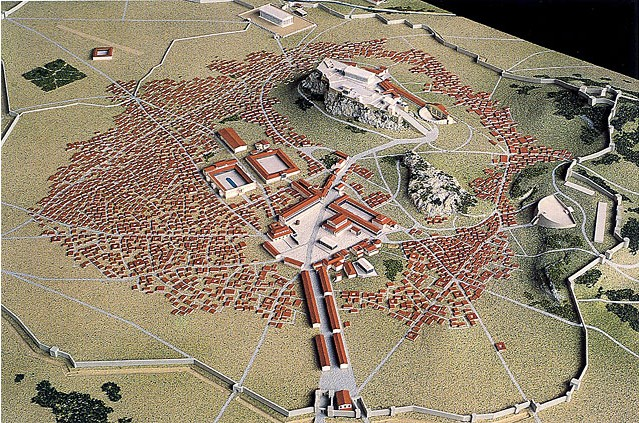
\includegraphics[width=10cm]{./figures/AtomId_1.png}
\caption{公元前2世纪雅典鸟瞰图} \label{AtomId_fig1}
\end{figure}

\subsection{柏拉图的四元素说}

关于物质的理论,自古就有,比如古希腊的泰勒斯曾说 “万物皆水”,后来又有人说万物是四种元素 “水、气、土、火” 构成.这就是所谓四元素说.

四元素说本来是古希腊人的常识(common sense),但柏拉图给这种关于物质的学说理论化,系统化了.这些内容被记载在柏拉图(427 BC — 347 BC)的宇宙论《蒂迈欧篇》中.

这里我们可以给出一个论证的概要:

\begin{itemize}
\item 万物或者是可见的,或者是可以触摸的.可见是因为光,可以触摸是因为坚硬.光是火的性质,坚硬是土的性质,这样我们就有了“火和土”两种元素.

\item 万物是三维的,我们需要像“胶水”一样的元素把“火和土”按比例混合起来成为三维的物体. 这里柏拉图是通过构造如下数列来论证的:
\begin{equation}
1=1^2=1^3, 2, 4=2^2, 8=2^3, 16=4^2, 32, 64=4^3,...
\end{equation}
这里$1=1^3$,$8=2^3$,$64=4^3$,...,叫做立方数. 每两个立方数之间正好是两个数,比如1和8之间是2和4;而8和64之间是16和32. 柏拉图因此论证说需要两种元素在“火和土”之间调和使生成万物,这两种元素就是水和气.

\item 不论是可见,还是可以触摸,都可以归结为形状,而形状可以归结为多边形的拼合,多边形则可以归结为三角形的拼合. 三角形是研究形的基础,或说三角形是研究几何学的基础.

\item 柏拉图提出了两种基本的直角三角形:(1)等腰直角三角形,记做$T_{45}$;(2)一个锐角为$30^o$的直角三角形,记做$T_{30}$.

\item 利用两种基本的直角三角形可以拼成四种正多面体,即正四面体、正八面体、正六面体和正二十面体.
\end{itemize}

\begin{figure}[ht]
\centering
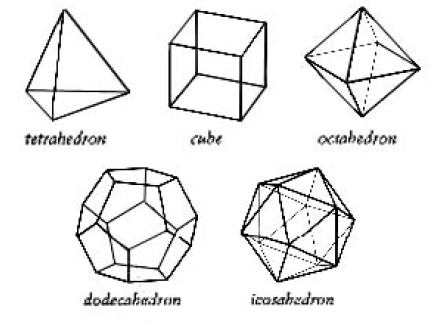
\includegraphics[width=8cm]{./figures/AtomId_2.png}
\caption{五种正多面体,也称柏拉图多面体.这里面的正十二面体没有出现在对元素的构造中,这是柏拉图理论中欠缺美感的地方.} \label{AtomId_fig2}
\end{figure}

\begin{enumerate}
\item 柏拉图认为立方体,即正六面体最稳定,因此把土的形定为正六面体.
\item 正四面体有最锐利的尖角,因此是最活跃的.火的形就是正四面体.
\item 剩下的还有气和水.因为气比水活跃,因此气的形就是正八面体.
\item 还剩下最后一个,正二十面体,是水的形.
\end{enumerate}

这些形都是很小的,用今天的话说就是“水气土火”的原子.并且这些原子还可以相互转化.

\begin{table}[ht]
\centering
\caption{柏拉图的“元素说”}\label{AtomId_tab1}
\begin{tabular}{|c|c|c|c|}
\hline
元素 & 正$n$面体 & 等腰直角三角形 & $30^o$直角三角形 \\
\hline
土 & 正六面体 & 12 & 0  \\
\hline
火 & 正四面体 & 0 & 8 \\
\hline
气 & 正八面体 & 0 & 16 \\
\hline
水 & 正二十面体 & 0 & 40\\
\hline
\end{tabular}
\end{table}

\begin{itemize}
\item 只有土是由等腰直角三角形围成的,因此土最稳定,它会被火溶解,可以被气或水分解,但不会转变成其它元素.

\item “火、气、水”都是由$30^o$的直角三角形围成的,因此可相互转换.比如,我们可以写出如下的反应方程式:
\end{itemize}

\begin{equation}
1 Water \to 2 Gas + 1 Fire 
\end{equation}

反应前有40个$T_{30}$,而反应后有$2 \times 16 + 8 = 40$个$T_{30}$.我们可以把上式与电解水的反应方程式比较:

\begin{equation}
2 H_2 O \to 2 H_2 \uparrow + O_2 \uparrow
\end{equation}

从思维的角度这是属于同一母型(Prototype)的.如果我们说古代思想会对近代科学有启迪作用,或我们说人总是在几种思维母型里打转转就毫不奇怪了.实际上量子力学的创建者,比如海森堡自幼就熟读《蒂迈欧篇》,如果说这些这些直观的图像会对他有潜移默化的影响可能并不夸张.

以上是柏拉图元素论的概要,当然这些都是非常粗糙的论证,而且经不起实验的定量检测,但元素之间可以互相转化,这个想法还是启迪了后来的炼金术,并最终导致了近代化学的出现.

\subsection{伊壁鸠鲁的原子论}

原子在古希腊语中不可再分的意思,这个不可再分固可以做物理上的拆分理解,亦可作逻辑上的不可再分(析)理解.比如刚才介绍的柏拉图关于“水气火土”四元素的理论就是逻辑上无法再分析的范例.

柏拉图的理论在古代是显学,2000多年来一直有稳定的传承,但它在古代并非没有对手,比如从德谟克利特、留基伯到伊壁鸠鲁、卢克莱修的原子论.但说实话这两种理论区别并不大,他们争执不休,以至于柏拉图都准备带弟子去焚烧德谟克利特的著作,并非是他们对自然真有什么本质的看法不同,毕竟都是一个时代对自然的看法.

关键的分歧是他们对伦理学和政治学的观点不一样,而古人的学问是个整体,伦理学的基础是哲学和科学,要驳倒对方,争取听众,釜底抽薪,攻击对方的科学观点是一个潜在的选择.

古代原子论者是今天所说的唯物论者,他们不相信灵魂,把生命看做是一堆原子具有功能性、活性或协调一致运动的集合.就好像是一把调谐良好的里拉琴,只要弦不断就能奏出美妙的音乐,对应于人的生命状态,而弦断则对应人亡,灵魂在这里是无所栖身的.没有灵魂,自然就没有死后世界,所有传统的道德说理就被架空了,Polis将处于危机之中.柏拉图派对唯物论者(或自然哲学家)的反感和敌对就在这里.

当然这并非我们现在的主题,我也不再继续展开讨论,而仅仅强调一点,即当我们讲到古代原子论的时候,我们应把柏拉图派的很多观点、理论也置于古代原子论的范畴内,而不仅仅是介绍自然哲学家的原子论.实际上很多柏拉图派的理念,比如天球的理念和近代原子模型是很接近的.对玻尔、海森堡这些哲学倾向很强的物理学家,很难想象他们没有阅读过《理想国》和《蒂迈欧篇》,而如果读过的话,他们一定对柏拉图的“数学-几何学”的宇宙模型印象深刻.

下面我将扼要地介绍伊壁鸠鲁的原子论,伊壁鸠鲁(341 BC — 270 BC)的《致希罗多德书信》是现存最早的关于原子论的记录,再早的比如德谟克利特和留基伯的就都已经失传了.

\begin{itemize}
\item 在视觉上存在最小的点,再小我们就看不见了,这个视觉上的最小的点是有大小的. 由此类比:物质也是由最小的不可再分的最小单元构成的,再小是不存在的.就这一点而言,伊壁鸠鲁的方案和柏拉图的方案是不同的,柏拉图的基础三角形没有明确地说存在最小、最基础的三角形.今天的人大多会认为物质存在最小的不可再分的单元是很抽象的,或很难想象,但在古人那里也许未必.比如在中国古代是通过计量“肥而美”的“黑小米”来建立度量衡制度的,而在古代西方也有类似的比喻,比如卢克莱修在《物性论》中把水想象为大量罂粟籽的集合,比如阿基米德在《数沙者》中假想整个宇宙都充满了沙子,然后计算了整个宇宙中有多少粒沙子.古人的数学观念是由 “1,2,3,……” 出发开始建立的,对他们来说想象一个由原子构成的世界其实是更简单的.这个原子就好比构成宇宙、万物的基础砖石,我们先寻求生命的结构和功能,进而问生命的可能的意义是什么?

\item 原子很小,因为我们谁也没见过原子.但我们没法假设原子的大小是绝对的0,因为如果那样的话,很多原子就无法构成万物了,而万物在我们的眼里是有体积的.

\item 原子如果有大小,那它就有部分,有形状.所以这里我们说的“不可再分”其实是物理意义下的,因为从几何学的角度,原子既然有部分,有形状,那它就可以在想象中继续分解.这里区分了物理意义下的“分”,和数学意义下的“分”.前者对应今天的原子物理和量子力学,而后者对应的则是数学分析.

\item 
原子既然有大小,有形状,它们之间就可以发生机械的相互作用,甚至结合成几个原子构成的具有特定功能的结构单元——分子.

没错,这都是伊壁鸠鲁天才的猜想.从字面上说已经很类似今天化学、甚至生物化学对结构和功能的解释.

当然,这里我们无需把这一天才的猜想神秘化,古代世界是个机械的世界,各种机械装置,从三列战舰、到攻城者德米特里乌斯的巨型攻城器械,古希腊人生活在这样一个机械无所不在的航海和贸易的时代,把原子想象成简单机械,把分子想象成具有特定功能的机械组合,进而把生命想象成极复杂的巨型机械都不是不可能的.
\end{itemize}

小结一下:柏拉图的四元素说和伊壁鸠鲁的原子论都是基于“形”的学说,但伊壁鸠鲁不能把他的理论数学化同时他的兴趣也不在于研究诸如——既然原子是有大小的,那么原子的大小到底是多少呢?——这类问题.

因此虽然古代原子论,无论是柏拉图的学说还是伊壁鸠鲁等自然哲学家的学说对人们想象原子有启发,但都不能说古希腊人已经接近了一个近代的原子论.近代原子论正如海森堡所说,是建立在一系列实验事实基础上的,当然还有概念体系和计算方法.

以下摘录海森堡在《物理学和哲学》第四章的一段讨论作为本小节的结束.

“在将原子物理学中的现代观点和希腊哲学作了类比之后,我们必须补充一个警告,即对这种类比不应有所误解.乍看起来,似乎希腊哲学家由于某种天才直觉而得到了与我们现代相同或很相似的结论,而我们的结论却是经过几个世纪的实验和数学方面的艰苦劳动才得到的.对我们的类比的这种解释无论如何是一种完全的误解.

在现代科学和希腊哲学之间有着巨大的差别,那就是现代科学的经验主义态度.自从伽利略和牛顿的时代以来,现代科学就已奠基于对自然的详细研究之上,奠基于这样一个假设之上,这就是:只有已被实验证实的或至少能被实验证实的陈述才是容许作出的.为了研究细节并在连续不断的变化中找到经久不变的定律,人们可用一个实验在自然中隔离出若干事件,这种观念希腊哲学家是没有想到过的.

由此可见,现代科学在一开始就立足于一个比古代哲学更谨慎同时也更巩固得多的基础之上.因此,现代物理学的陈述在某种意义上比希腊哲学更严肃得多.”

\subsection{三角学}

\subsubsection{角度}

首先由圆出发,假设圆的半径是$R$,角$\theta$张成的圆弧是$l$.

\begin{figure}[ht]
\centering
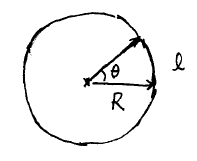
\includegraphics[width=4.5cm]{./figures/AtomId_3.png}
\caption{圆} \label{AtomId_fig3}
\end{figure}

\begin{equation}
l = R \theta
\end{equation}

这其实构成了对角度$\theta$的定义,

\begin{equation}
\theta = \frac{l }{R }
\end{equation}

假想这个圆以半径$R$完整地转一圈,我们把这个角度定义为$2 \pi$,在平面上的张角只能取$0 \to 2 \pi$,$\pi$是个无理数,它近似地等于:

\begin{equation}
\pi = 3.14159265 ...
\end{equation}

这样定义的角度叫“弧度制”.但通常我们会把一个完整的圆周分成完全相等的360份,每一份称为一度,一度再等分为60份,每份叫一分,一分再等分为60份,每份叫1秒,这就是所谓“度分秒”制.

“度分秒制”的好处是,60很容易被2、3、4、5、6等分,这对古人精确地计算星星在天空中的方位是很重要的.比如:17度25分30秒可记为:

\begin{equation}
17^o 25' 30''
\end{equation}

我们可以把一个圆周对应的张角分成完全相等的四份,每一份都是个直角,一个直角在弧度制下是 $\pi/2$,而在度分秒制下则是$90^o$.

\subsubsection{正弦和余弦函数}

现在来考虑一个直角三角形,即一个角是直角的三角形:

\begin{figure}[ht]
\centering
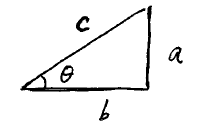
\includegraphics[width=4.5cm]{./figures/AtomId_4.png}
\caption{直角三角形} \label{AtomId_fig4}
\end{figure}

假设其中一个锐角是$\theta$,$\theta$所对的直角边是$a$,另一条直角边是$b$,斜边是$c$,我们有毕达哥拉斯定理:“斜边的平方等于两直角边的平方和”.

\begin{equation}
c^2 = a^2 + b^2
\end{equation}

我们可定义正弦和余弦函数如下:

\begin{equation}
\sin \theta = \frac{a}{c} \qquad
\cos \theta = \frac{b}{c}
\end{equation}

即正弦函数被定义为对边$a$与斜边$c$之比,而余弦函数被定义为邻边$b$和斜边$c$之比.

\begin{figure}[ht]
\centering
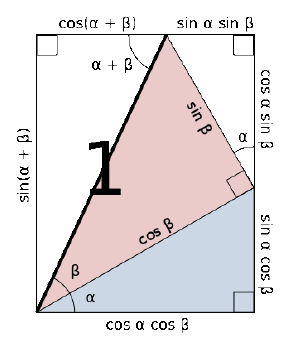
\includegraphics[width=6cm]{./figures/AtomId_5.png}
\caption{两角和公式} \label{AtomId_fig5}
\end{figure}

类似地我们还可定义正切函数($\tan \theta$)和余切函数($\cot \theta$):

\begin{equation}
\begin{aligned}
\tan \theta & = \frac{a}{b} \\
\cot \theta & = \frac{b}{a}
\end{aligned}
\end{equation}

现在考虑一个单位圆,即半径为1的圆,假设圆上一点逆时针地围绕圆心转动起来.这一点向$x$轴的投影是$x$,向$y$轴的投影是$y$.

\begin{figure}[ht]
\centering
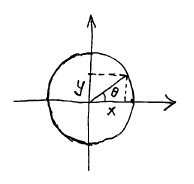
\includegraphics[width=5cm]{./figures/AtomId_6.png}
\caption{投影} \label{AtomId_fig6}
\end{figure}

据说第一个三角函数表(Trigonometric table)是古希腊天文学家伊巴古(又译作喜帕恰斯,190-125 BC)编纂的.

\begin{table}[ht]
\centering
\caption{常见三角函数的取值}\label{AtomId_tab2}
\begin{tabular}{|c|c|c|}
\hline
$\theta$ & $\sin \theta$ &  $\cos \theta$ \\
\hline
0  &  0 &  1 \\
\hline
$\pi/4$ & $\frac{1}{\sqrt 2}$  & $\frac{1}{\sqrt 2}$ \\
\hline
$\pi/2$ & 1  &  0 \\
\hline
$\pi$ & 0 & -1 \\
\hline
\end{tabular}
\end{table}

根据上表,我们可以计算:

\begin{equation}
\begin{aligned}
\sin ( \theta + \pi /2) & = \sin \theta \cos \pi /2 + \cos \theta  \sin \pi/2 = \cos \theta \\
\cos ( \theta + \pi /2) & = \cos  \theta \cos \pi /2 - \sin \theta \sin \pi/2 = - \sin \theta
\end{aligned}
\end{equation}

于是得到正弦/余弦函数的性质:

\begin{equation}
\begin{aligned}
\sin ( \theta + \pi /2 ) & = \cos \theta \\
\cos ( \theta + \pi /2) & = - \sin \theta
\end{aligned}
\end{equation}

当$\theta$从$0 \to 2\pi$变化时,$x$的取值将从$1 \to 0 \to -1 \to 0 \to 1$,然后重复,而$y$的取值将从$0 \to 1 \to 0 \to -1 \to 0$,然后重复.

\begin{figure}[ht]
\centering
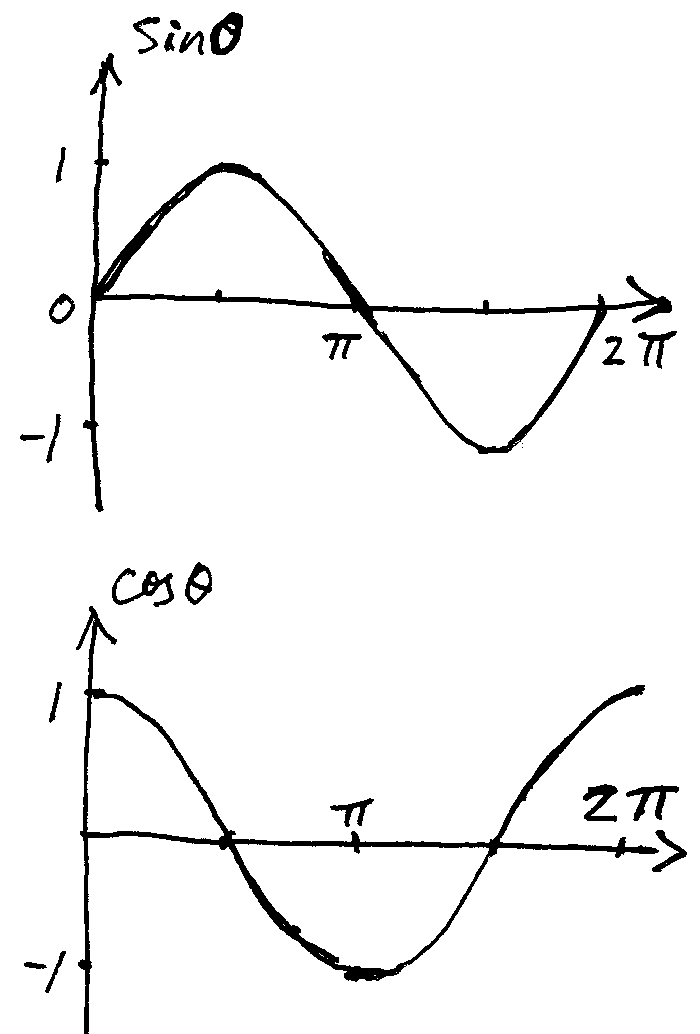
\includegraphics[width=5cm]{./figures/AtomId_7.png}
\caption{$\sin\theta$ 和 $\cos\theta$} \label{AtomId_fig7}
\end{figure}


这种周期性的运动很类似月相的变化,望是满月,朔是新月,由于月球围绕地球的运动,我们在地球上观察将看到月亮由月初的新月,到月中(十五)的满月,然后到月末又回到新月,然后重复.

在此意义下我们称$\theta$为相位(phase).

正弦和余弦函数在物理学中的用处很多,比如它是弹簧振子的解,是波动方程的解等.

\subsubsection{振动}

对振动而言,相位是:

\begin{equation}
\theta = \omega t 
\end{equation}

这里$\omega$叫角频率,当$\omega t = 2 \pi$时,振动正好重复一个周期$T$,

\begin{equation}
T = \frac{2 \pi}{\omega}
\end{equation}

描述振动的方程是:

\begin{equation}
A \cos \omega t
\end{equation}

$A$叫做振幅,振动将在$A \to 0 \to -A \to 0 \to A$重复发生.

\begin{table}[ht]
\centering
\caption{$A \cos \omega t$ 描述的运动}\label{AtomId_tab3}
\begin{tabular}{|c|c|c|}
\hline
时间 & 相位 &  位置 \\
\hline
0 & 0 & A \\
\hline
T/4 & $\pi /2 $ & 0 \\
\hline
T/2 & $\pi$ & -A \\
\hline
3T/4 & $3 \pi /2  $ &  0 \\
\hline
T &  $2\pi$  & A \\
\hline
\end{tabular}
\end{table}

但有时候当$t = 0$时,我们就已经有了一个非零的相位$\theta_0$了,这时描述振动的方程将变成:

\begin{equation}
A \cos (\omega t + \theta_0)
\end{equation}

这里$\theta_0$叫做初相位(initial phase),我们管用正弦/余弦函数描述的振动叫简谐振动.


\subsubsection{波动}

振动是在时间变量上的重复.波动是在时间和空间上的重复.我们所处的世界是一维的时间再加上三维的空间.为了简单,我们先考虑空间也是一维的情况.

假设我们在体育场里造人浪(Mexican wave),开始的时候也许只有一个人重复地做“站起-欢呼-坐下”,再“站起-欢呼”再“坐下”,然后重复的动作,他旁边紧挨着的人注意到他的动作,也会跟着模仿他的动作,但因为距离的存在,旁边的人要反应过来跟着他一起做需要过一段时间,即有个时间的延迟.

\begin{figure}[ht]
\centering
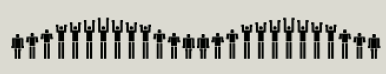
\includegraphics[width=7cm]{./figures/AtomId_8.png}
\caption{墨西哥人浪起源于1986年的墨西哥世界杯.在那届世界杯上,热情的球迷自发地运用一种交替起立欢呼的方式自娱自乐,为球队加油,从远处看就像一阵阵的海浪.} \label{AtomId_fig8}
\end{figure}


假设人与人之间的间距是$\Delta x$,时间的延迟是$\Delta t$,波动在空间上传播的速度就是:

\begin{equation}
v = \frac{\Delta x }{\Delta t}
\end{equation}

假设第一个人正好完成了一个振动的周期$T$: “坐着、站起、欢呼、坐下、坐着”

这时如果他抬头看的话,他会发现距离他$\lambda$远处某个人正处于和他一样“坐着”的状态,而且他马上就要站起来了,因为他紧邻的人已经在做“站起”的动作了.

可以设想,这两个相距$\lambda$的人将做完全同步的振动,在我们外人看来,他们一起“坐着”,又一起“站起”,一起“欢呼”,……

如果用振动的语言说的话,它们的相位是相同的.但这么说让我们不舒服,因为毕竟后一个人的运动要晚于第一个人,我们说,“空间相距$\lambda$远的两个点,它们运动的相位正好差$2 \pi$”.


这样说就舒服了.

现在我们假设体育场里已经造起了人浪,我们应该如何描述它呢?这是一个以空间位置$x$和时间$t$为变量的函数.

假设$t$固定,比如令$t = 0$我们得到一个随$x$起伏变化的函数,这就相当于是照相机照的快照,在某个时间运动冻结了,但仍会在空间$x$上有个分布,假设这个函数是:

\begin{equation}
\psi (x, t = 0) 
\end{equation}

这个分布其实就是个波形,它围绕$x = 0$附近展开.单独看这个随$x$起伏的波形,它也是周期性的,是空间调制意义下的周期性,每增加波长$\lambda$,$\psi$就重复.

假设$\psi$可以表示为一个正弦/余弦函数,这意味着:$x$每增加$\lambda$,相位的变化是$2 \pi$.即:

\begin{equation}
\psi (x, t = 0) = A \cos \frac{2 \pi x}{ \lambda}
\end{equation}

\begin{figure}[ht]
\centering
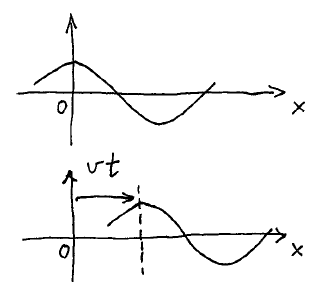
\includegraphics[width=5cm]{./figures/AtomId_9.png}
\caption{经过时间$t$,波形会向前移动$vt$,或者说是函数沿$x$方向发生了平移,平移前函数是$\psi(x)$,而平移后函数是$\psi(x - vt)$.} \label{AtomId_fig9}
\end{figure}

现在假设时间是$t$,并且$t > 0$,波形会向前传播,时间$t$波形向前移动了$vt$,这意味着波函数是在$x = vt$附近展开的.

\begin{equation}
\psi(x,t) = A \cos \frac{2 \pi}{\lambda} \left( x - vt \right)
\end{equation}

假设波形移动$\lambda$需要花费时间$T$,波形移动的速度$v$是:

\begin{equation}
v = \frac{\lambda}{ T }
\end{equation}

波函数$\psi(x,t)$变成:

\begin{equation}
\psi(x, t) = A \cos   2\pi \left(  \frac{x}{\lambda} - \frac{t}{T}   \right)
\end{equation}

定义波矢$k$,和角频率$\omega$分别为:

\begin{equation}
\begin{aligned}
k &= \frac{2 \pi}{\lambda} \\
\omega &= \frac{2 \pi}{T}
\end{aligned}
\end{equation}

波函数取常见的形式:

\begin{equation}
\psi (x,t )= A \cos \left( k x - \omega t \right)
\end{equation}

现在相位是:

\begin{equation}
k x - \omega t
\end{equation}

固定时间,我们会得到波动随空间的分布,$x$越大,相位也越大.固定位置,我们会得到波动就在这个位置随时间的振动.

\begin{exercise}{}
假设人眼瞳孔大小是 $2\Si{mm}$,可见光波长是 $550\Si{nm}$,利用公式:

\begin{equation}
\theta = 1.22 \cdot \frac{\lambda}{D}
\end{equation}

估算人眼的角分辨本领,并把结果换算为“度分秒”为单位.

据说第谷(1546-1601)对星星观察的准确度能够达到二弧分,已经逼近肉眼的理论极限,当然夜晚观星瞳孔会放大,这有利于提高他的精度.
\end{exercise}
